\documentclass[8pt]{beamer}

% Beamer style
%\usetheme[secheader]{Madrid}
% \usetheme{CambridgeUS}
\useoutertheme{infolines}
\usecolortheme[rgb={0.65,0.15,0.25}]{structure}
% \usefonttheme[onlymath]{serif}
\beamertemplatenavigationsymbolsempty
%\AtBeginSubsection

% Packages
%\usepackage[french]{babel}
\usepackage[latin1]{inputenc}
\usepackage{color}
\usepackage{xspace}
\usepackage{dsfont, stmaryrd}
\usepackage{amsmath, amsfonts, amssymb, stmaryrd}
\usepackage{epsfig}
\usepackage{tikz}
\usepackage{url}
% \usepackage{ulem}
\usepackage{astats}
%\usepackage[all]{xy}
\usepackage{graphicx}
\usepackage{xspace}
\usepackage{pifont}
\usepackage{marvosym}

% Maths
% \newtheorem{theorem}{Theorem}
% \newtheorem{definition}{Definition}
\newtheorem{proposition}{Proposition}
% \newtheorem{assumption}{Assumption}
% \newtheorem{algorithm}{Algorithm}
% \newtheorem{lemma}{Lemma}
% \newtheorem{remark}{Remark}
% \newtheorem{exercise}{Exercise}
% \newcommand{\propname}{Prop.}
% \newcommand{\proof}{\noindent{\sl Proof:}\quad}
% \newcommand{\eproof}{$\blacksquare$}

% \setcounter{secnumdepth}{3}
% \setcounter{tocdepth}{3}
\newcommand{\pref}[1]{\ref{#1} p.\pageref{#1}}
\newcommand{\qref}[1]{\eqref{#1} p.\pageref{#1}}

% Colors : http://latexcolor.com/
\definecolor{darkred}{rgb}{0.65,0.15,0.25}
\definecolor{darkgreen}{rgb}{0,0.4,0}
\definecolor{darkred}{rgb}{0.65,0.15,0.25}
\definecolor{amethyst}{rgb}{0.6, 0.4, 0.8}
\definecolor{asparagus}{rgb}{0.53, 0.66, 0.42}
\definecolor{applegreen}{rgb}{0.55, 0.71, 0.0}
\definecolor{awesome}{rgb}{1.0, 0.13, 0.32}
\definecolor{blue-green}{rgb}{0.0, 0.87, 0.87}
\definecolor{red-ggplot}{rgb}{0.52, 0.25, 0.23}
\definecolor{green-ggplot}{rgb}{0.42, 0.58, 0.00}
\definecolor{purple-ggplot}{rgb}{0.34, 0.21, 0.44}
\definecolor{blue-ggplot}{rgb}{0.00, 0.49, 0.51}

% Commands
\newcommand{\backupbegin}{
   \newcounter{finalframe}
   \setcounter{finalframe}{\value{framenumber}}
}
\newcommand{\backupend}{
   \setcounter{framenumber}{\value{finalframe}}
}
\newcommand{\emphase}[1]{\textcolor{darkred}{#1}}
\newcommand{\comment}[1]{\textcolor{gray}{#1}}
\newcommand{\paragraph}[1]{\textcolor{darkred}{#1}}
\newcommand{\refer}[1]{{\small{\textcolor{gray}{{\cite{#1}}}}}}
\newcommand{\Refer}[1]{{\small{\textcolor{gray}{{[#1]}}}}}
\newcommand{\goto}[1]{{\small{\textcolor{blue}{[\#\ref{#1}]}}}}
\renewcommand{\newblock}{}

\newcommand{\tabequation}[1]{{\medskip \centerline{#1} \medskip}}
% \renewcommand{\binom}[2]{{\left(\begin{array}{c} #1 \\ #2 \end{array}\right)}}

% Variables 
\newcommand{\Abf}{{\bf A}}
\newcommand{\Beta}{\text{B}}
\newcommand{\Bcal}{\mathcal{B}}
\newcommand{\Bias}{\xspace\mathbb B}
\newcommand{\Cor}{{\mathbb C}\text{or}}
\newcommand{\Cov}{{\mathbb C}\text{ov}}
\newcommand{\cl}{\text{\it c}\ell}
\newcommand{\Ccal}{\mathcal{C}}
\newcommand{\cst}{\text{cst}}
\newcommand{\Dcal}{\mathcal{D}}
\newcommand{\Ecal}{\mathcal{E}}
\newcommand{\Esp}{\xspace\mathbb E}
\newcommand{\Espt}{\widetilde{\Esp}}
\newcommand{\Covt}{\widetilde{\Cov}}
\newcommand{\Ibb}{\mathbb I}
\newcommand{\Fcal}{\mathcal{F}}
\newcommand{\Gcal}{\mathcal{G}}
\newcommand{\Gam}{\mathcal{G}\text{am}}
\newcommand{\Hcal}{\mathcal{H}}
\newcommand{\Jcal}{\mathcal{J}}
\newcommand{\Lcal}{\mathcal{L}}
\newcommand{\Mt}{\widetilde{M}}
\newcommand{\mt}{\widetilde{m}}
\newcommand{\Nbb}{\mathbb{N}}
\newcommand{\Mcal}{\mathcal{M}}
\newcommand{\Ncal}{\mathcal{N}}
\newcommand{\Ocal}{\mathcal{O}}
\newcommand{\pt}{\widetilde{p}}
\newcommand{\Pt}{\widetilde{P}}
\newcommand{\Pbb}{\mathbb{P}}
\newcommand{\Pcal}{\mathcal{P}}
\newcommand{\Qcal}{\mathcal{Q}}
\newcommand{\qt}{\widetilde{q}}
\newcommand{\Rbb}{\mathbb{R}}
\newcommand{\Sbb}{\mathbb{S}}
\newcommand{\Scal}{\mathcal{S}}
\newcommand{\st}{\widetilde{s}}
\newcommand{\St}{\widetilde{S}}
\newcommand{\Tcal}{\mathcal{T}}
\newcommand{\todo}{\textcolor{red}{TO DO}}
\newcommand{\Ucal}{\mathcal{U}}
\newcommand{\Un}{\math{1}}
\newcommand{\Vcal}{\mathcal{V}}
\newcommand{\Var}{\mathbb V}
\newcommand{\Vart}{\widetilde{\Var}}
\newcommand{\Zcal}{\mathcal{Z}}

% Symboles & notations
\newcommand\independent{\protect\mathpalette{\protect\independenT}{\perp}}\def\independenT#1#2{\mathrel{\rlap{$#1#2$}\mkern2mu{#1#2}}} 
\renewcommand{\d}{\text{\xspace d}}
\newcommand{\gv}{\mid}
\newcommand{\ggv}{\, \| \, }
% \newcommand{\diag}{\text{diag}}
\newcommand{\card}[1]{\text{card}\left(#1\right)}
\newcommand{\trace}[1]{\text{tr}\left(#1\right)}
\newcommand{\matr}[1]{\boldsymbol{#1}}
\newcommand{\matrbf}[1]{\mathbf{#1}}
\newcommand{\vect}[1]{\matr{#1}} %% un peu inutile
\newcommand{\vectbf}[1]{\matrbf{#1}} %% un peu inutile
\newcommand{\trans}{\intercal}
\newcommand{\transpose}[1]{\matr{#1}^\trans}
\newcommand{\crossprod}[2]{\transpose{#1} \matr{#2}}
\newcommand{\tcrossprod}[2]{\matr{#1} \transpose{#2}}
\newcommand{\matprod}[2]{\matr{#1} \matr{#2}}
\DeclareMathOperator*{\argmin}{arg\,min}
\DeclareMathOperator*{\argmax}{arg\,max}
\DeclareMathOperator{\sign}{sign}
\DeclareMathOperator{\tr}{tr}
\newcommand{\ra}{\emphase{$\rightarrow$} \xspace}

% Hadamard, Kronecker and vec operators
\DeclareMathOperator{\Diag}{Diag} % matrix diagonal
\DeclareMathOperator{\diag}{diag} % vector diagonal
\DeclareMathOperator{\mtov}{vec} % matrix to vector
\newcommand{\kro}{\otimes} % Kronecker product
\newcommand{\had}{\odot}   % Hadamard product

% TikZ
\newcommand{\nodesize}{2em}
\newcommand{\edgeunit}{2.5*\nodesize}
\newcommand{\edgewidth}{1pt}
\tikzstyle{node}=[draw, circle, fill=black, minimum width=.75\nodesize, inner sep=0]
\tikzstyle{square}=[rectangle, draw]
\tikzstyle{param}=[draw, rectangle, fill=gray!50, minimum width=\nodesize, minimum height=\nodesize, inner sep=0]
\tikzstyle{hidden}=[draw, circle, fill=gray!50, minimum width=\nodesize, inner sep=0]
\tikzstyle{hiddenred}=[draw, circle, color=red, fill=gray!50, minimum width=\nodesize, inner sep=0]
\tikzstyle{observed}=[draw, circle, minimum width=\nodesize, inner sep=0]
\tikzstyle{observedred}=[draw, circle, minimum width=\nodesize, color=red, inner sep=0]
\tikzstyle{eliminated}=[draw, circle, minimum width=\nodesize, color=gray!50, inner sep=0]
\tikzstyle{empty}=[draw, circle, minimum width=\nodesize, color=white, inner sep=0]
\tikzstyle{blank}=[color=white]
\tikzstyle{nocircle}=[minimum width=\nodesize, inner sep=0]

\tikzstyle{edge}=[-, line width=\edgewidth]
\tikzstyle{edgebendleft}=[-, >=latex, line width=\edgewidth, bend left]
\tikzstyle{edgebendright}=[-, >=latex, line width=\edgewidth, bend right]
\tikzstyle{lightedge}=[-, line width=\edgewidth, color=gray!50]
\tikzstyle{lightedgebendleft}=[-, >=latex, line width=\edgewidth, bend left, color=gray!50]
\tikzstyle{lightedgebendright}=[-, >=latex, line width=\edgewidth, bend right, color=gray!50]
\tikzstyle{edgered}=[-, line width=\edgewidth, color=red]
\tikzstyle{edgebendleftred}=[-, >=latex, line width=\edgewidth, bend left, color=red]
\tikzstyle{edgebendrightred}=[-, >=latex, line width=\edgewidth, bend right, color=red]

\tikzstyle{arrow}=[->, >=latex, line width=\edgewidth]
\tikzstyle{arrowbendleft}=[->, >=latex, line width=\edgewidth, bend left]
\tikzstyle{arrowbendright}=[->, >=latex, line width=\edgewidth, bend right]
\tikzstyle{arrowred}=[->, >=latex, line width=\edgewidth, color=red]
\tikzstyle{arrowbendleftred}=[->, >=latex, line width=\edgewidth, bend left, color=red]
\tikzstyle{arrowbendrightred}=[->, >=latex, line width=\edgewidth, bend right, color=red]
\tikzstyle{arrowblue}=[->, >=latex, line width=\edgewidth, color=blue]
\tikzstyle{dashedarrow}=[->, >=latex, dashed, line width=\edgewidth]
\tikzstyle{dashededge}=[-, >=latex, dashed, line width=\edgewidth]
\tikzstyle{dashededgebendleft}=[-, >=latex, dashed, line width=\edgewidth, bend left]
\tikzstyle{lightarrow}=[->, >=latex, line width=\edgewidth, color=gray!50]

\newcommand{\BEDD}{BEDD\xspace}
\newcommand{\fignet}{/home/robin/RECHERCHE/RESEAUX/EXPOSES/FIGURES}

%==================================================================
%==================================================================
\begin{document}
%==================================================================
%==================================================================
\title{Motifs and bipartite networks}
\author{S. Robin}
\institute[Sorbonne universit\'e]{\normalsize{Sorbonne universit\'e}}
\date[EcoNet, Apr'24]{Ecole EcoNet, April 2024, Montpellier}
\maketitle

%==================================================================
\frame{\frametitle{Outline} \tableofcontents}

%==================================================================
%==================================================================
\section{Bipartite networks and motifs}
\frame{\frametitle{Outline} \tableofcontents[currentsection]}%==================================================================
\frame{\frametitle{Bipartite network}

  \begin{tabular}{ll}
    \begin{tabular}{p{.45\textwidth}}
      \paragraph{Two types of actors.}
      \begin{itemize}
      \item Mutualistic: plant-pollinator
      \item Antagonistic: host-parasite
      \end{itemize}
      \bigskip \bigskip 
      \paragraph{Topological analysis:} \\
      understanding the network organisation \\
      \bigskip
      \paragraph{Local:} % \\
      node or edge properties (degree, betweenness) \\
      \bigskip
      \paragraph{Global:} % \\
      density, connected components, nestedness 
    \end{tabular}
    &
    \begin{tabular}{p{.45\textwidth}}
      \paragraph{Zackenberg network: } 
      \refer{SRO16} \\
      \includegraphics[width=.4\textwidth, trim=0 50 0 50]{\fignet/Zackenberg-1996_12-red-net} \\
%       \includegraphics[width=.4\textwidth, trim=0 50 0 50]{\fignet/Zackenberg-1996_12-red-adj}
    \end{tabular} 
  \end{tabular}
}

%==================================================================
\frame{\frametitle{Bipartite network: notations}

  \begin{tabular}{ll}
    \begin{tabular}{p{.6\textwidth}}
      \paragraph{Species.}
      \begin{itemize}
        \setlength{\itemsep}{1.15\baselineskip}
        \item $i = 1, \dots m$ insects = rows = bottom nodes
        \item $j = 1, \dots n$ plants = columns = top nodes
      \end{itemize}
    \end{tabular}
    &
    \hspace{-.15\textwidth}
    \begin{tabular}{p{.4\textwidth}}
      \includegraphics[width=.4\textwidth, trim=0 50 0 50]{\fignet/Zackenberg-1996_12-red-net} 
    \end{tabular} 
    \\ \pause
    \begin{tabular}{p{.6\textwidth}}
      \paragraph{Interactions.}
      \begin{itemize}
      \item $A_{ij} = 1$ if insect $i$ interacts with plant $j$, \\
      0 otherwise
      $$
      A_{ij} = 1 \quad \Leftrightarrow \quad i \sim j
      $$
      \item adjacency matrix : $m \times n$
      $$
      A = [A_{ij}]_{1 \leq i \leq m, 1 \leq j \leq n}
      $$
      \end{itemize}
    \end{tabular}
    &
    \hspace{-.15\textwidth}
    \begin{tabular}{p{.5\textwidth}}
      \includegraphics[width=.4\textwidth, trim=0 50 0 50]{\fignet/Zackenberg-1996_12-red-adj}
    \end{tabular} 
  \end{tabular}
}

%==================================================================
\frame{\frametitle{Bipartite motifs}

  \begin{tabular}{ll}
    \hspace{-.04\textwidth}
    \begin{tabular}{p{.45\textwidth}}
      \paragraph{'Meso-scale' analysis.} \refer{SCB19}
      \begin{itemize}
       \item Motifs ='building-blocks'
       \item between local (several nodes) and global (sub-graph)
      \end{itemize}
      \bigskip \bigskip 
      \onslide+<2->{
      \paragraph{Interest.}
      \begin{itemize}
       \item Generic description of a network
       \item Enables network comparison
       \item Even when the nodes are different
      \end{itemize} \\
      ($+$ 'species-role': out of the scope here) \\
      }
      \bigskip \bigskip 
      \onslide+<3->{
      \paragraph{Existing tool.} 
      \url{bmotif} package \refer{SSS19}: \\
      counts motif occurrences
      }
    \end{tabular}
    &
    \begin{tabular}{p{.45\textwidth}}
      \hspace{-0.035\textwidth}
      \includegraphics[width=.5\textwidth]{\fignet/SCB19-Oikos-Fig3-6motifs} \\      
    \end{tabular} 
  \end{tabular}

}

%==================================================================
\frame{\frametitle{Example}

  \begin{tabular}{ll}
    \begin{tabular}{p{.45\textwidth}}
      \paragraph{Plant-pollinator network} \refer{SRO16} \\
      \hspace{-.05\textwidth}
      \includegraphics[width=.45\textwidth, trim=0 50 0 50]{\fignet/Zackenberg-1996_12-red-net} \\
    \end{tabular}
    &
    \begin{tabular}{p{.45\textwidth}}
      \paragraph{Motif counts.}  \\ ~\\ 
      4 nodes (species) \\ 
      \includegraphics[width=.09\textwidth]{\fignet/Zackenberg-1996_12-red-motif5} 
      \includegraphics[width=.09\textwidth]{\fignet/Zackenberg-1996_12-red-motif6} \\ ~\\
      5 nodes \\ 
      \includegraphics[width=.09\textwidth]{\fignet/Zackenberg-1996_12-red-motif9} 
      \includegraphics[width=.09\textwidth]{\fignet/Zackenberg-1996_12-red-motif10} 
      \includegraphics[width=.09\textwidth]{\fignet/Zackenberg-1996_12-red-motif11} 
      \includegraphics[width=.09\textwidth]{\fignet/Zackenberg-1996_12-red-motif12} \\
      \includegraphics[width=.09\textwidth]{\fignet/Zackenberg-1996_12-red-motif13} 
      \includegraphics[width=.09\textwidth]{\fignet/Zackenberg-1996_12-red-motif14} 
      \includegraphics[width=.09\textwidth]{\fignet/Zackenberg-1996_12-red-motif15} 
      \includegraphics[width=.09\textwidth]{\fignet/Zackenberg-1996_12-red-motif16} 
    \end{tabular}  
    ~ \\
    \hline
    \\
    \begin{tabular}{p{.45\textwidth}}
      top 'stars' (plants) \\
      \includegraphics[width=.09\textwidth]{\fignet/Zackenberg-1996_12-red-motif1} 
      \includegraphics[width=.09\textwidth]{\fignet/Zackenberg-1996_12-red-motif2} 
      \includegraphics[width=.09\textwidth]{\fignet/Zackenberg-1996_12-red-motif7} 
      \includegraphics[width=.09\textwidth]{\fignet/Zackenberg-1996_12-red-motif17} 
    \end{tabular}
    &    
    \begin{tabular}{p{.45\textwidth}}
      bottom 'stars' (pollinators) \\
      \includegraphics[width=.09\textwidth]{\fignet/Zackenberg-1996_12-red-motif1} 
      \includegraphics[width=.09\textwidth]{\fignet/Zackenberg-1996_12-red-motif3} 
      \includegraphics[width=.09\textwidth]{\fignet/Zackenberg-1996_12-red-motif4} 
      \includegraphics[width=.09\textwidth]{\fignet/Zackenberg-1996_12-red-motif8} 
    \end{tabular}
  \end{tabular}
  
}

%==================================================================
%==================================================================
\section{A null model}
\frame{\frametitle{Outline} \tableofcontents[currentsection]}%==================================================================
\frame{\frametitle{Need for a null model}

  \paragraph{Motif counts} obviously depend on 
  \begin{itemize}
   \item the \emphase{size} of the network: $n \times m$
   \item the \emphase{density} of the network
   \item the \emphase{imbalance} between bottom-node degrees (specialist vs generalist insects)
   \item the \emphase{imbalance} between top-node degrees (specialist vs generalist plants)
  \end{itemize}
  
  \bigskip \bigskip \pause
  \paragraph{Bipartite expected degree distribution (\BEDD) model:} (in words)
  \begin{itemize}
    \setlength{\itemsep}{1.15\baselineskip}
    \item Consider $m$ insects ($i = 1, \dots m$): \\
    each plant $i$ has a specific propensity to interact (degree of generalism)
    \item Consider $n$ plants ($j = 1, \dots n$): \\
    each plant $j$ has a specific propensity to interact  (idem)
    \item The probability for insect $i$ and plant $j$ to interact is proportional to the product of their respective propensities.
  \end{itemize}

}

%==================================================================
\frame{\frametitle{\BEDD model}

  \paragraph{Bipartite expected degree distribution (\BEDD) model:} (more formaly)
  \begin{itemize}
    \setlength{\itemsep}{1.15\baselineskip}
    \item $\rho =$ network density
    \item $g =$ top node degree imbalance ($\int g = 1$)
    \item $h =$ bottom node degree imbalance ($\int h = 1$)
  \end{itemize}
  
  $$
  \{U_i\}_{i = 1, \dots m} \text{ iid } \sim \Ucal[0, 1] 
  \qquad \qquad 
  \{V_j\}_{j = 1, \dots n} \text{ iid } \sim \Ucal[0, 1]
  $$
  
  $$
  \Pbb\{i \sim j \mid U_i, V_j\} = \emphase{\rho \; g(U_i) \; h(V_j)}
  $$ 

  \bigskip
  (Bipartite version of the EDD model \refer{ChL02})

}

%==================================================================
\frame{\frametitle{\BEDD model}

  \begin{tabular}{cccc}
    & & $h_0(v) =$ & $h(v) =$ \\
    \multicolumn{2}{c}{
      $\begin{array}{rl}
        \Pbb\{i \sim j \mid U_i, V_j\} & = \rho \; g(U_i) \; h(V_j) \\ \\
        \Esp (D_i \mid U_i) & = n \; \rho \; g(U_i) \\ \\
        \Esp (D_j \mid V_j) & = m \; \rho \; g(V_i) 
      \end{array}$
    } &
    \begin{tabular}{c} 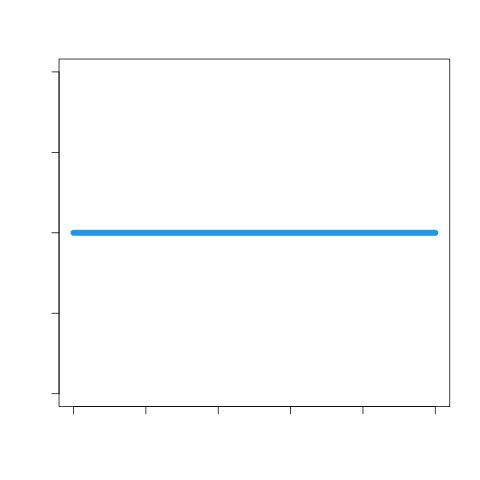
\includegraphics[width=.18\textwidth]{\fignet/FigMotifsBEDD-dist-h10} \end{tabular} &
    \begin{tabular}{c} 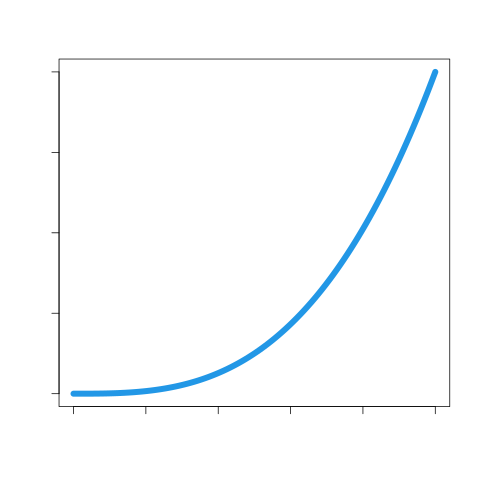
\includegraphics[width=.18\textwidth]{\fignet/FigMotifsBEDD-dist-h40} \end{tabular} \\
    \begin{tabular}{c} $g_0(u) =$ \end{tabular} &
    \begin{tabular}{c} 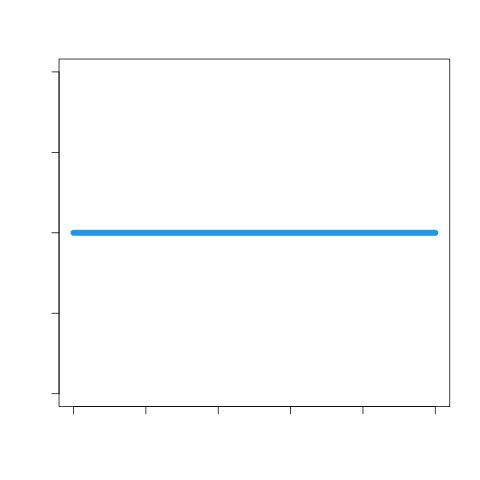
\includegraphics[width=.18\textwidth]{\fignet/FigMotifsBEDD-dist-g10} \end{tabular} &
    \begin{tabular}{c} 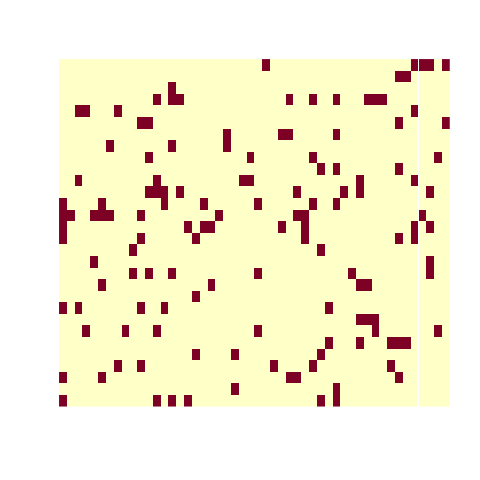
\includegraphics[width=.18\textwidth]{\fignet/FigMotifsBEDD-adj-g10-h10} \end{tabular} &
    \begin{tabular}{c} 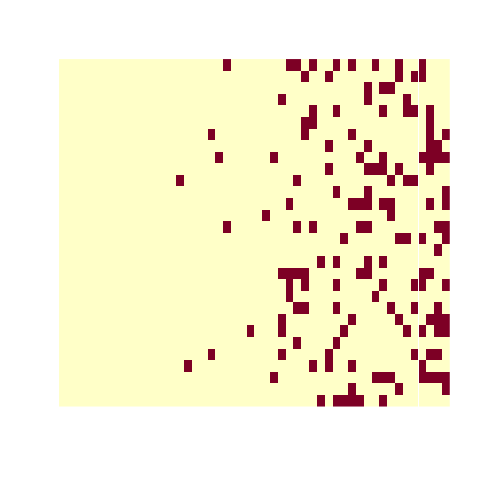
\includegraphics[width=.18\textwidth]{\fignet/FigMotifsBEDD-adj-g10-h40} \end{tabular} \\
    \begin{tabular}{c} $g(u) =$ \end{tabular} &
    \begin{tabular}{c} 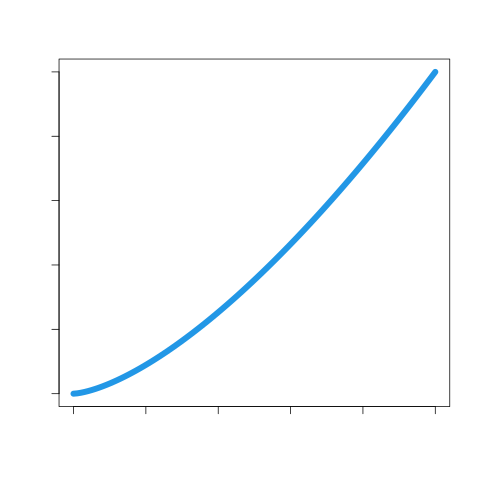
\includegraphics[width=.18\textwidth]{\fignet/FigMotifsBEDD-dist-g25} \end{tabular} &
    \begin{tabular}{c} 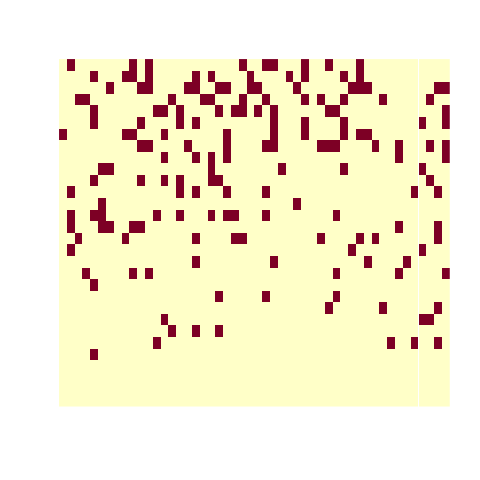
\includegraphics[width=.18\textwidth]{\fignet/FigMotifsBEDD-adj-g25-h10} \end{tabular} &
    \begin{tabular}{c} 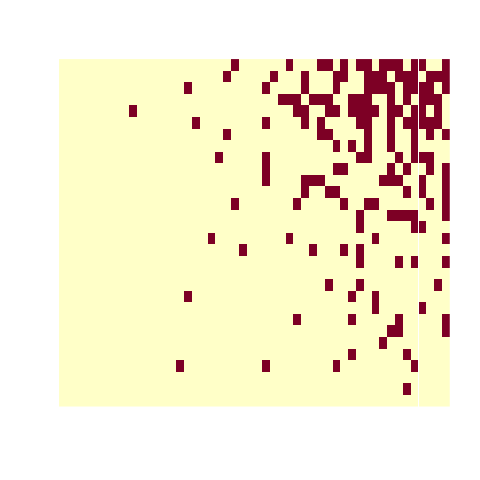
\includegraphics[width=.18\textwidth]{\fignet/FigMotifsBEDD-adj-g25-h40} \end{tabular} \\
  \end{tabular}
  
}

%==================================================================
\frame{\frametitle{Properties of the \BEDD model}

  \paragraph{Assumptions.}
  \begin{itemize}
    \setlength{\itemsep}{1\baselineskip}
    \item No preferred or avoided specific connexion
    \item \emphase{Graph-exchangeable} model: insects and plants can be permuted simultaneously
  \end{itemize}
  
  \bigskip \bigskip \pause
  \paragraph{Properties.}
  \begin{itemize}
    \setlength{\itemsep}{1\baselineskip}
    \item Expected degree for insect $i$ given $U_i$ : $n \; g(U_i)$.
    \item Expected degree for plant $j$ given $V_j$ : $m \; h(V_j)$.
    \item 'Nested' structure by construction
  \end{itemize}
  
  \bigskip \bigskip \pause
  \paragraph{Sufficient statistics} to fit \BEDD: 
  \begin{itemize}
    \setlength{\itemsep}{1\baselineskip}
    \item Insect degrees + plant degrees
    \item or, equivalently, star (single edge, top, bottom) frequencies
  \end{itemize}

  }

%==================================================================
%==================================================================
\section{Motif distribution}
\frame{\frametitle{Outline} \tableofcontents[currentsection]}%==================================================================
\frame{\frametitle{Counting motifs}

  \hspace{-.05\textwidth}
  \begin{tabular}{ll}
    \begin{tabular}{p{.4\textwidth}}
      \paragraph{Number of positions.}
      \begin{itemize}
       \item Choose $p$ nodes among $m$
       \item Choose $q$ nodes among $n$
       \item Try all {\sl automorphisms} 
      \end{itemize}
      $$
      c_s := 
      \left(\begin{array}{c}m \\ p\end{array}\right)
      \times \left(\begin{array}{c}n \\ q\end{array}\right)
      \times r_s
      $$ 
      ~ \\ ~ \\
    \end{tabular}
    & \pause
    \begin{tabular}{p{.5\textwidth}}
      \paragraph{Automorphisms=} non-redundant permutations \\
      \includegraphics[width=.1\textwidth]{\fignet/FigMotifsBEDD-motif9-automorphism1}
      \includegraphics[width=.1\textwidth]{\fignet/FigMotifsBEDD-motif9-automorphism2}
      \includegraphics[width=.1\textwidth]{\fignet/FigMotifsBEDD-motif9-automorphism3} \\
      \includegraphics[width=.1\textwidth]{\fignet/FigMotifsBEDD-motif9-automorphism4}
      \includegraphics[width=.1\textwidth]{\fignet/FigMotifsBEDD-motif9-automorphism5}
      \includegraphics[width=.1\textwidth]{\fignet/FigMotifsBEDD-motif9-automorphism6} 
    \end{tabular} 
  \end{tabular}
  
  \bigskip \bigskip \pause
  \paragraph{Motif count.} Try all positions $\alpha = 1, \dots c_s$, define 
  $$
  Y_{s\alpha} = 1 \text{ if match,} \qquad 0 \text{ otherwise},
  $$
  then count the number of matches:
  $$
  N_s = \sum_\alpha Y_{s\alpha}
  $$
  \ra \emphase{Motif frequency}: $F_s := N_s / c_s$
  
}

%==================================================================
\frame{\frametitle{Motif probability}

  \paragraph{Occurrence probability $\overline{\phi}_s = \Pbb\{Y_{s\alpha} = 1\}$.} Under the B-EDD model \refer{OLR22}:
  \begin{align*}
    \overline{\phi}_s 
    & :=
    \Pbb_{\BEDD}\left(
    \includegraphics[width=.06\textwidth, trim=100 200 100 0]{\fignet/FigMotifsBEDD-motif9} 
    \right)
    \; = \; 
    \frac{
    \onslide+<2->{
      \overset{\text{top stars}}{\overbrace{
      \Pbb\left(\includegraphics[width=.05\textwidth, trim=100 200 100 0]{\fignet/FigMotifsBEDD-motif9-top1}\right) % \times 
      \Pbb\left(\includegraphics[width=.05\textwidth, trim=100 200 100 0]{\fignet/FigMotifsBEDD-motif9-top1}\right) % \times 
      \Pbb\left(\includegraphics[width=.05\textwidth, trim=100 200 100 0]{\fignet/FigMotifsBEDD-motif9-top2}\right)   }}
    }
    \onslide+<3->{
      \times
      \overset{\text{bottom stars}}{\overbrace{
      \Pbb\left(\includegraphics[width=.05\textwidth, trim=100 200 100 0]{\fignet/FigMotifsBEDD-motif9-bottom1}\right) % \times
      \Pbb\left(\includegraphics[width=.05\textwidth, trim=100 200 100 0]{\fignet/FigMotifsBEDD-motif9-bottom3}\right)
      }}
    }
    }{
    \onslide+<4->{
      \underset{\text{edges}}{\underbrace{
      \left(\Pbb\left(\includegraphics[width=.05\textwidth, trim=100 200 100 0]{\fignet/FigMotifsBEDD-motif9-top1}\right)\right)^4
      }}
    }
    } 
    \\
    \onslide+<5->{
    & =
    \frac{\phi_1^2 \phi_2 \phi_1 \phi_4}{\phi_1^4}
    \qquad =
    \frac{\phi_2 \phi_4}{\phi_1}
    }
  \end{align*}

  \onslide+<6->{\bigskip \bigskip 
  \paragraph{Estimated probability.} 
  $$
  \overline{\phi}_s := \frac{\phi_2 \phi_4}{\phi_1}
  \qquad \rightarrow \qquad 
  \overline{F}_s := \frac{F_2 F_4}{F_1}
  $$
  where $F_1$, $F_2$, $F_4 =$ observed frequencies of  edges, top stars and bottom stars.
  }
}

%==================================================================
\frame{\frametitle{Moments of the count}

  \begin{itemize}
  \setlength{\itemsep}{1.5\baselineskip}
  \item \emphase{Mean:} $\Esp_{\BEDD}(N_s) = c_s \times \overline{\phi}_s$ 
  \item \pause \emphase{Variance:} Same game, requires to evaluate $\displaystyle{\Esp_{\BEDD}(N_s ^2) = \Esp_{\BEDD}\left(\sum_\alpha Y_{s\alpha} \right)^2}$ \\
  \ra Need to account for overlap between positions ({\sl super-motifs}: \refer{PDK08}) 
  $$
  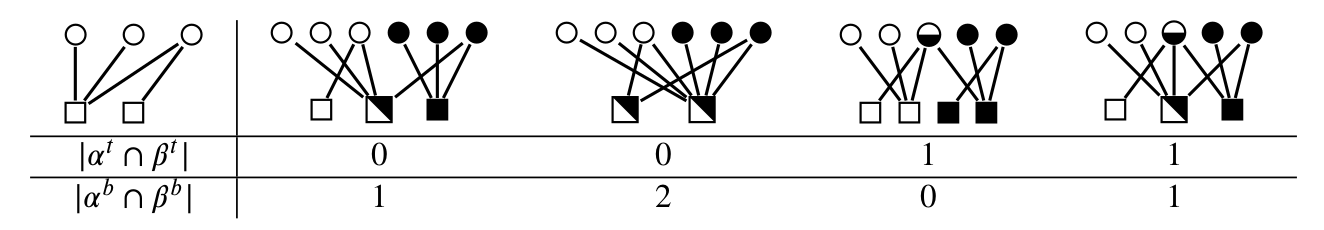
\includegraphics[width=.8\textwidth, trim=0 25 0 0, clip=]{\fignet/OLR22-EJS-Fig2}
  $$ \\ ~
  \item \pause \emphase{Covariance:} Same game to compute $\Cov(N_s, N_{s'})$
  \end{itemize}

}

%==================================================================
\frame{\frametitle{Distribution of the count}

  \paragraph{Asymptotic normality for non-star motifs.} Under \BEDD (and sparsity conditions):
  $$
  (F_s - \overline{F}_s) \left/ \sqrt{\widehat{\Var}(F_s)} \right. \quad \overset{m, n \rightarrow \infty}{\longrightarrow} \quad \Ncal(0, 1)
  $$
  Proof \refer{OLR22}: 
  \begin{equation*}
    \text{decompose} \qquad
   F_s - \overline{F}_s 
   = \underset{\text{random fluctuations}}{\underbrace{(F_s - \phi_s)}} 
   + \underset{\text{null under \BEDD}}{\underbrace{(\phi_s - \overline{\phi}_s)}}  
   + \underset{\text{estimation error } \rightarrow 0}{\underbrace{(\overline{\phi}_s - \overline{F}_s)}}, 
  \end{equation*}
  + construct a counting martingale for $F_s - \phi_s$  \refer{GaL17b}.
  
  \bigskip \bigskip \pause
  \paragraph{Consequence.} We know the expected behavior of motif counts under the BEDD model (= 'null model').
}

%==================================================================
%==================================================================
\section{Goodness-of-fit and network comparison}
\frame{\frametitle{Outline} \tableofcontents[currentsection]}%==================================================================
\frame{\frametitle{Goodness-of-fit (GOF)}

  \paragraph{Aim.} Test if the observed data arise from a given model.

  \medskip
  More cautious: 'if the model fits the data reasonably well'
  
  \bigskip \bigskip \pause
  \paragraph{Typical approach.} 
  \begin{enumerate}
    \setlength{\itemsep}{1.15\baselineskip}
    \item Define some statistic (= function of the data) $T$, 
    \item Establish the distribution of $T$ under the model, 
    \item Compare the observed value of $T$ with its distribution under the model.
  \end{enumerate}

  
  \bigskip \bigskip \pause
  \paragraph{Example.} 
  \begin{enumerate}
    \item Data = observed plant-pollinator network
    \item Statistic $T$ = motif count $N_s$ 
    \item Model = BEDD
  \end{enumerate}

}

%==================================================================
\frame{\frametitle{Goodness-of-fit (GOF) of the BEDD model}

  \hspace{-.05\textwidth}
  \begin{tabular}{ll}
    \begin{tabular}{p{.5\textwidth}}
      \onslide+<1->{\paragraph{Raw statistic:}
      $$
      T_s = \frac{N_s - \widehat{\Esp} N_s}{\sqrt{\widehat{\Var} N_s}}
      $$ \\ 
      }
      \onslide+<2->{
      \paragraph{Corrected stat.:} accounts for the estimation error in $\widehat{\Esp} N$
      $$
      T'_s = \frac{N_s - (\widehat{\Esp} N_s - \emphase{\widehat{\Bias}(\widehat{\Esp} N_s)})}{\sqrt{\emphase{\widehat{\Var} (N_s - \widehat{\Esp} N_s)}}}
      $$ \\ 
      }
%       \onslide+<3>{\paragraph{Choleski\footnote{$\Sigma = P \Lambda P^\intercal$, $\Sigma = P \Lambda^{-1/2} P^\intercal$} transformation:} accounts for the correlation between the counts
%       $$
%       \Sigma_{s, s'} = \Cov(N_s - \widehat{\Esp} N_s, N_{s'} - \widehat{\Esp} N_{s'})
%       $$
%       $$
%       T'' = \emphase{\widehat{\Sigma}^{-1/2}}
%       \left[N_s - (\widehat{\Esp} N_s - \widehat{\Bias}(\widehat{\Esp} N_s))\right]
%       $$
%       }
    \end{tabular}
    &
    \begin{tabular}{p{.4\textwidth}}
      \hspace{-.05\textwidth}
      \onslide+<1->{\paragraph{Zackenberg network.} ~ \\}
      \begin{overprint}
        \onslide<1>
        \includegraphics[width=.4\textwidth]{\fignet/Zackenberg-1996_12-red-StatCount}
        \onslide<2>
        \includegraphics[width=.4\textwidth]{\fignet/Zackenberg-1996_12-red-NormStatCount}
%         \onslide<3>
%         \includegraphics[width=.4\textwidth]{\fignet/Zackenberg-1996_12-red-CholNormStat}
      \end{overprint}
    \end{tabular} 
  \end{tabular}

}

%==================================================================
\frame{\frametitle{Testing degree imbalance}

  \paragraph{Question.} Is there some degree imbalance between plants?
  
  \bigskip \pause
  \paragraph{Statistical test.} 
  \begin{itemize}
    \item Assume $A \sim BEDD(\rho, g, h)$, 
    $$
    H_0 = \{h = 1\}
    $$
    \item For motif $s$, evaluate $\widehat{\Esp}_0(N_s)$ and $\widehat{\Esp}_0(N_s)$ and compare 
    $$
    W_s = (N_s - \widehat{\Esp}_0(N_s)) / \sqrt{\widehat{\Var}_0(N_s)}
    $$ 
    with $\Ncal(0, 1)$
  \end{itemize}

  
  \bigskip \pause
  \paragraph{Example.} (only one significant difference) 
  $$
  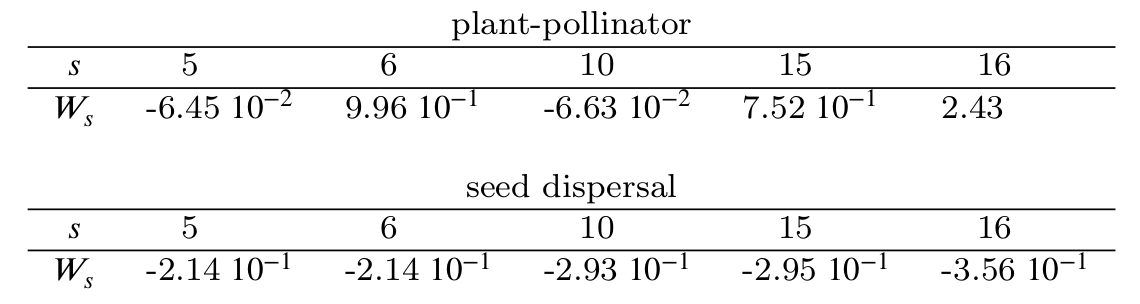
\includegraphics[width=.75\textwidth]{\fignet/OLR22-EJS-Tab3}
  $$
}


%==================================================================
\frame{\frametitle{Comparing network imbalances}

  \paragraph{Question.} Do network $A$ and $B$ share the same imbalance for insects?
  
  \bigskip \pause
  \paragraph{Statistical test.} 
  \begin{itemize}
    \item Assume $A \sim BEDD(\rho^A, g^A, h^A)$ and $B \sim BEDD(\rho^B, g^B, h^B)$
    $$
    H_0 = \{g^A = g^B\}
    $$
    \item For motif $s$, evaluate $\widehat{\Esp}_{\widehat{\rho}^A, \emphase{\widehat{g}^B}, \widehat{g}^A}(N^A_s)$ and $\widehat{\Esp}_{\widehat{\rho}^B, \emphase{\widehat{g}^A}, \widehat{g}^B}(N^B_s)$ and compare 
    $$
    W_s = \frac{(N_s^A - \widehat{\Esp}_0(N_s^A)) - (N_s^B - \widehat{\Esp}_0(N_s^B))}{\sqrt{\widehat{\Var}_0(N^A_s) + \widehat{\Var}_0(N^B_s)}}
    $$ 
    with $\Ncal(0, 1)$
  \end{itemize}

  
  \bigskip \pause
  \paragraph{Example.} (no significant difference) 
  $$
  \includegraphics[width=.8\textwidth]{\fignet/OLR22-EJS-Tab4}
  $$

}

%==================================================================
%==================================================================
\section{Network embedding}
\frame{\frametitle{Outline} \tableofcontents[currentsection]}%==================================================================
\frame{\frametitle{Network embedding: Multivariate analysis}

  \paragraph{Analysing multiple networks.} Principle
  \begin{itemize}
   \item 'Embed' each network into a convenient space (e.g. $\Rbb^d$)
   \item Use standard multivariate analysis (clustering, PCA, MDS, ...)
  \end{itemize}
  
  \bigskip \bigskip \pause
  \paragraph{Using motifs.} $K$ networks 
  $$
  (\text{Network})_k \quad \rightarrow \quad
  (N^k_1, \dots, N^k_S) \in \Rbb^S
  $$
  but need to correct for: network sizes, correlation between motif frequencies, etc...

  \bigskip \bigskip \pause
  \hspace{-.05\textwidth}
  \begin{tabular}{ll}
    \begin{tabular}{p{.4\textwidth}}
      \paragraph{~Zackenberg dataset.} $K = 46$ networks 
      \begin{itemize}
      \item 2 years
      \item 1 network observed every few days 
      \end{itemize}
    \end{tabular}
    &
    \begin{tabular}{p{.5\textwidth}}
      \includegraphics[width=.1\textwidth]{\fignet/Zackenberg-red-96:5-adj}
      \includegraphics[width=.1\textwidth]{\fignet/Zackenberg-red-96:10-adj}
      \includegraphics[width=.1\textwidth]{\fignet/Zackenberg-red-96:15-adj} 
      \includegraphics[width=.1\textwidth]{\fignet/Zackenberg-red-96:20-adj} 
      \dots \\
      \includegraphics[width=.1\textwidth]{\fignet/Zackenberg-red-97:5-adj}
      \includegraphics[width=.1\textwidth]{\fignet/Zackenberg-red-97:10-adj}
      \includegraphics[width=.1\textwidth]{\fignet/Zackenberg-red-97:15-adj} 
      \includegraphics[width=.1\textwidth]{\fignet/Zackenberg-red-97:20-adj} 
      \dots
    \end{tabular} 
  \end{tabular}

}

%==================================================================
\frame{\frametitle{Choleski transform}

  \bigskip
  \paragraph{Aim:} 'Remove' correlation and variance heterogeneity
  
  \bigskip
  \begin{tabular}{cc}
    \hspace{-0.04\textwidth}
    \begin{tabular}{p{.45\textwidth}}
      \paragraph{Covariance matrix $(X_1, X_2)$:}
      $$
      \Sigma(X_1, X_2) = \left[\begin{array}{cc} 
                      \sigma^2_1 & \sigma_{12} \\
                      \sigma_{12} & \sigma^2_2 \\
                     \end{array}\right]
      $$
    \end{tabular}
    & 
    \begin{tabular}{p{.45\textwidth}}
      \onslide+<2->{\paragraph{Choleski transform:}
      $$
      \left[\begin{array}{c} X'_1 \\ X'_2 \end{array} \right]
      = \Sigma^{-1/2} \left[\begin{array}{c} X_1 \\ X_2 \end{array} \right]
      $$}
    \end{tabular} 
    \\
    \hspace{-0.04\textwidth}
    \begin{tabular}{c}
      \vspace{-0.08\textheight}
      \includegraphics[width=0.35\textwidth, trim=25 25 25 25, clip=]{\fignet/Cholevski-raw} 
    \end{tabular}
    & 
    \begin{tabular}{c}
      \vspace{-0.08\textheight}
      \onslide+<2->{\includegraphics[width=0.35\textwidth, trim=25 25 25 25, clip=]{\fignet/Cholevski-chol}}
    \end{tabular} 
    \\
    \hspace{-0.04\textwidth}
    \begin{tabular}{p{.45\textwidth}}
      Diagonalization: $\Sigma = P \emphase{\Lambda} P^{-1}$ \\
      ~ \\
      Choleski matrix: $\Sigma^{-1/2} = P \emphase{\Lambda^{-1/2}} P^{-1}$
    \end{tabular}
    & \pause
    \begin{tabular}{p{.45\textwidth}}
      \onslide+<2->{$$
      \Sigma(X'_1, X'_2) = \left[\begin{array}{cc} 
                      1 & 0 \\
                      0 & 1 \\
                     \end{array}\right]
      $$}
    \end{tabular} 
  \end{tabular}

}

%==================================================================
\frame{\frametitle{Network embedding: Zackenberg's data \refer{SRO16}}

  \bigskip
  \begin{tabular}{c|c|c|c}
    \onslide+<1->{Raw counts} & 
    \onslide+<2->{Corrected stat.} & 
    \onslide+<3->{Choleski} & 
    \onslide+<4>{Bray-Curtis MDS} \\
    \hline
    \onslide+<1->{\includegraphics[width=.2\textwidth, height=.175\textheight]{\fignet/Zackenberg-red-PCAcount-scree}} &
    \onslide+<2->{\includegraphics[width=.2\textwidth, height=.175\textheight]{\fignet/Zackenberg-red-PCAstat-scree}} & 
    \onslide+<3->{\includegraphics[width=.2\textwidth, height=.175\textheight]{\fignet/Zackenberg-red-PCAchol-scree}} &  
    \onslide+<4>{\includegraphics[width=.2\textwidth, height=.175\textheight]{\fignet/Zackenberg-red-MDSBrayCurtis-scree}}
    \\
    \onslide+<1->{\includegraphics[width=.22\textwidth]{\fignet/Zackenberg-red-PCAcount-biplot}} &
    \onslide+<2->{\includegraphics[width=.22\textwidth]{\fignet/Zackenberg-red-PCAstat-biplot}} &
    \onslide+<3->{\includegraphics[width=.22\textwidth]{\fignet/Zackenberg-red-PCAchol-biplot}} &
    \onslide+<4>{\includegraphics[width=.22\textwidth]{\fignet/Zackenberg-red-MDSBrayCurtis-biplot}}
    \\
    \onslide+<1->{\includegraphics[width=.2\textwidth]{\fignet/Zackenberg-red-PCAcount-size}} &
    \onslide+<2->{\includegraphics[width=.2\textwidth]{\fignet/Zackenberg-red-PCAstat-size}} &
    \onslide+<3->{\includegraphics[width=.2\textwidth]{\fignet/Zackenberg-red-PCAchol-size}} &
    \onslide+<4>{\includegraphics[width=.2\textwidth]{\fignet/Zackenberg-red-MDSBrayCurtis-size}}
  \end{tabular}

}

% %==================================================================
% \frame{\frametitle{Contrast-based network embedding}
%   \todo{on-going work with Natasha}
% }


%====================================================================
\frame[allowframebreaks]{ \frametitle{References}
  {%\footnotesize
   \tiny
   \bibliography{/home/robin/Biblio/BibGene}
%    \bibliographystyle{/home/robin/LATEX/Biblio/astats}
   \bibliographystyle{alpha}
  }
}

%==================================================================
%==================================================================
\backupbegin
%==================================================================
\frame{\frametitle{Super-motifs}

  \begin{tabular}{ll}
    \begin{tabular}{p{.4\textwidth}}
      \paragraph{Motif:}
      $$
      \includegraphics[width=.1\textwidth, ]{\fignet/FigMotifsBEDD-motif9}
      $$
      ~\\ ~\\
      \paragraph{Variance:}
      $$
      \begin{array}{rcl}
        N_s^2 & = & \displaystyle{\left(\sum_\alpha Y_{s\alpha}\right)^2} \\
        ~ \\
        & = & \displaystyle{\sum_{\alpha, \beta: \alpha \cap \beta = \emptyset} Y_{s\alpha} Y_{s\beta}} \\
        ~ \\
        & & \displaystyle{+ \sum_{\alpha, \beta: \alpha \cap \beta \neq \emptyset} \underset{\footnotesize\begin{array}{c}\text{occurrence of} \\ \text{a super-motif} \end{array}}{\underbrace{Y_{s\alpha} Y_{s\beta}}}} \\
      \end{array}
      $$
    \end{tabular} 
    &
    \begin{tabular}{p{.5\textwidth}}
      \paragraph{Some super-motifs:} \\
      \includegraphics[width=.1\textwidth, ]{\fignet/FigMotifsBEDD-motif9-supermotif1} 
      \includegraphics[width=.1\textwidth, ]{\fignet/FigMotifsBEDD-motif9-supermotif2} 
      \includegraphics[width=.1\textwidth, ]{\fignet/FigMotifsBEDD-motif9-supermotif3} 
      \includegraphics[width=.1\textwidth, ]{\fignet/FigMotifsBEDD-motif9-supermotif4} \\
      \includegraphics[width=.1\textwidth, ]{\fignet/FigMotifsBEDD-motif9-supermotif5} 
      \includegraphics[width=.1\textwidth, ]{\fignet/FigMotifsBEDD-motif9-supermotif6} 
      \includegraphics[width=.1\textwidth, ]{\fignet/FigMotifsBEDD-motif9-supermotif7} 
      \includegraphics[width=.1\textwidth, ]{\fignet/FigMotifsBEDD-motif9-supermotif8} \\
      \includegraphics[width=.1\textwidth, ]{\fignet/FigMotifsBEDD-motif9-supermotif9} 
      \includegraphics[width=.1\textwidth, ]{\fignet/FigMotifsBEDD-motif9-supermotif10}
      \includegraphics[width=.1\textwidth, ]{\fignet/FigMotifsBEDD-motif9-supermotif11}
      \includegraphics[width=.1\textwidth, ]{\fignet/FigMotifsBEDD-motif9-supermotif12} \\
      \includegraphics[width=.1\textwidth, ]{\fignet/FigMotifsBEDD-motif9-supermotif13} 
      \includegraphics[width=.1\textwidth, ]{\fignet/FigMotifsBEDD-motif9-supermotif14}
      \includegraphics[width=.1\textwidth, ]{\fignet/FigMotifsBEDD-motif9-supermotif15}
      \includegraphics[width=.1\textwidth, ]{\fignet/FigMotifsBEDD-motif9-supermotif16} \\
      ~ \\
      \dots 396 super-motifs \\
      ~ \\ ~ \\ ~ \\ 
    \end{tabular} 
  \end{tabular}
  
  \paragraph{Covariance:} same game, for $Y_{s\alpha} Y_{s'\beta}$ with $s \neq s'$

}

%==================================================================
\frame{\frametitle{Asymptotic distribution of the count}

  \bigskip 
  \paragraph{Estimated probability.} 
  $$
  \overline{\phi}_s := {\phi_2 \phi_4} \left/ {\phi_1} \right.
  \qquad \rightarrow \qquad 
  \overline{F}_s := {F_2 F_4} \left/ {F_1} \right.
  $$
  where $F_1$, $F_2$, $F_4 =$ observed frequencies of top stars, bottom stars and edges.
  
  \bigskip \bigskip \pause
  \paragraph{Asymptotic normality for non-star motifs.} Under \BEDD (and sparsity conditions):
  $$
  (F_s - \overline{F}_s) \left/ \sqrt{\widehat{\Var}(F_s)} \right. \quad \overset{m, n \rightarrow \infty}{\longrightarrow} \quad \Ncal(0, 1)
  $$
  Proof: 
  \begin{itemize}
   \item decompose 
   $$
   F_s - \overline{F}_s 
   = \underset{\text{random fluctuations}}{\underbrace{(F_s - \phi_s)}} 
   + \underset{\text{null under \BEDD}}{\underbrace{(\phi_s - \overline{\phi}_s)}}  
   + \underset{\text{estimation error } \rightarrow 0}{\underbrace{(\overline{\phi}_s - \overline{F}_s)}}, 
   $$
   \item construct a counting martingale \refer{GaL17b} for $F_s - \phi_s$
  \end{itemize}

  \bigskip \pause
  \paragraph{Test statistic.} Under \BEDD:
  $$
  N_s \approx \Ncal\left(\widehat{\Esp}(N_s), \widehat{\Var}(N_s)\right)
  \qquad  \Leftrightarrow \qquad 
  \left({N_s - \widehat{\Esp}(N_s)}\right)\left/{\sqrt{\widehat{\Var}(N_s)}}\right. \approx \Ncal\left(0, 1\right)
  $$
}

%==================================================================
\frame{\frametitle{In practice: Asymptotic normality}

  \begin{center}
  \begin{tabular}{cccc}
    ($n = 2m/3$) & $m=50$ & $m=100$ & $m=200$ \\
    \includegraphics[width=.1\textwidth]{\fignet/FigMotifsBEDD-adjMatMotif6} & 
    \includegraphics[width=.2\textwidth]{\fignet/FigMotifsBEDD-SimMotifBEDD-m50-n33-rho5-g2-h3-6nodesFALSE-B500-distCountMotif6} &
    \includegraphics[width=.2\textwidth]{\fignet/FigMotifsBEDD-SimMotifBEDD-m100-n67-rho5-g2-h3-6nodesFALSE-B500-distCountMotif6} &
    \includegraphics[width=.2\textwidth]{\fignet/FigMotifsBEDD-SimMotifBEDD-m200-n133-rho5-g2-h3-6nodesFALSE-B500-distCountMotif6} \\
    \includegraphics[width=.1\textwidth]{\fignet/FigMotifsBEDD-adjMatMotif16} & 
    \includegraphics[width=.2\textwidth]{\fignet/FigMotifsBEDD-SimMotifBEDD-m50-n33-rho5-g2-h3-6nodesFALSE-B500-distCountMotif16} &
    \includegraphics[width=.2\textwidth]{\fignet/FigMotifsBEDD-SimMotifBEDD-m100-n67-rho5-g2-h3-6nodesFALSE-B500-distCountMotif16} &
    \includegraphics[width=.2\textwidth]{\fignet/FigMotifsBEDD-SimMotifBEDD-m200-n133-rho5-g2-h3-6nodesFALSE-B500-distCountMotif16} \\
  \end{tabular}
  \end{center}
  
  \bigskip
  \textcolor{blue}{Normal} distribution, \textcolor{magenta}{Poisson-geometric} distribution with same mean and variance \refer{Sta01,PDK08}

}

%==================================================================
\frame{\frametitle{In practice: Test statistic}

  \paragraph{Need to account for the estimation error} of $\widehat{\Esp} N$
  
  \begin{center}
  \begin{tabular}{lccc}
    & $m=50$ & $m=100$ & $m=200$ \\
    \begin{tabular}{p{.175\textwidth}}
    Regular stat.: 
    $$
    {\frac{N - \widehat{\Esp} N}{\sqrt{\widehat{\Var} N}}}
    $$
    \end{tabular}
    & 
    \begin{tabular}{c}
    \includegraphics[width=.2\textwidth]{\fignet/FigMotifsBEDD-SimMotifBEDD-m50-n33-rho5-g2-h3-6nodesFALSE-B500-distRawStat6}
    \end{tabular}
    & 
    \begin{tabular}{c}
    \includegraphics[width=.2\textwidth]{\fignet/FigMotifsBEDD-SimMotifBEDD-m100-n67-rho5-g2-h3-6nodesFALSE-B500-distRawStat6}
    \end{tabular}
    & 
    \begin{tabular}{c}
    \includegraphics[width=.2\textwidth]{\fignet/FigMotifsBEDD-SimMotifBEDD-m200-n133-rho5-g2-h3-6nodesFALSE-B500-distRawStat6}
    \end{tabular}
    \\ \pause
    \begin{tabular}{p{.175\textwidth}}
    Correction: 
    $$
    {\frac{N - (\widehat{\Esp} N - \emphase{\widehat{\Bias}(\widehat{\Esp} N)})}{\sqrt{\emphase{\widehat{\Var} (N - \widehat{\Esp} N)}}}}
    $$
    \end{tabular}
    & 
    \begin{tabular}{c}    
    \includegraphics[width=.2\textwidth]{\fignet/FigMotifsBEDD-SimMotifBEDD-m50-n33-rho5-g2-h3-6nodesFALSE-B500-distNormStat6}
    \end{tabular}
    & 
    \begin{tabular}{c}
    \includegraphics[width=.2\textwidth]{\fignet/FigMotifsBEDD-SimMotifBEDD-m100-n67-rho5-g2-h3-6nodesFALSE-B500-distNormStat6}
    \end{tabular}
    & 
    \begin{tabular}{c}    
    \includegraphics[width=.2\textwidth]{\fignet/FigMotifsBEDD-SimMotifBEDD-m200-n133-rho5-g2-h3-6nodesFALSE-B500-distNormStat6}
    \end{tabular}
  \end{tabular}
  \end{center}
  
  \begin{itemize}
   \item Need to evaluate \emphase{$\Var(N - \widehat{\Esp}(N))$} and \emphase{$\Bias(\widehat{\Esp} N)$}: resort to Taylor expansion ($\Delta-$method)
  \end{itemize}
}

%==================================================================
%==================================================================
\backupend

%==================================================================
%==================================================================
\end{document}
%==================================================================
%==================================================================

\begin{tabular}{ll}
  \begin{tabular}{p{.45\textwidth}}
  \end{tabular}
  &
  \begin{tabular}{p{.45\textwidth}}
  \end{tabular} 
\end{tabular}
